\documentclass[]{article}
\usepackage{tikz}
\usepackage{todonotes}
\usetikzlibrary{calc,positioning,fit,arrows}
\title{Network of Habenula}
\author{Dilawar Singh}

\begin{document}
\maketitle


Synapse \tikz \draw[-*] (0,0) -- ++(.5,0); are excitatory, and synapse \tikz
\draw[-|,] (0,0) -- ++(.5,0); is inhibitory.

\begin{figure}[ht]
    \centering
    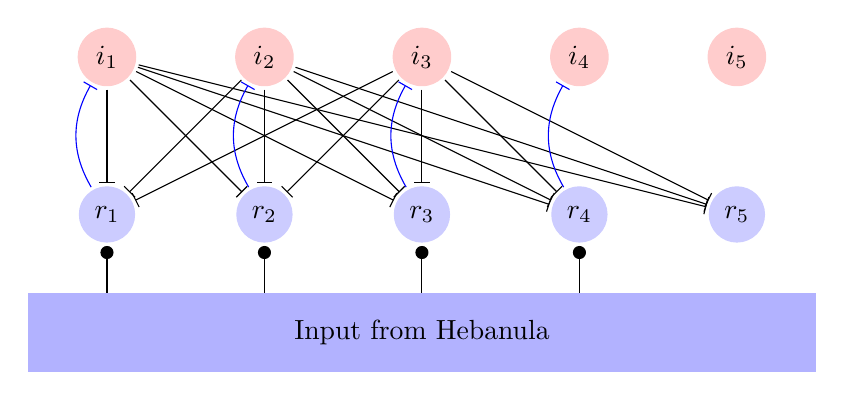
\begin{tikzpicture}[scale=1 
        , node distance = 2cm
        , every path/.style={ thin, draw, outer sep=.5mm }
        , every node/.style={  } 
        ]

        \foreach \y in {1,2,3,4,5} 
            \node[draw=red!20,circle,fill=red!20] (i\y) at (2*\y,0) {$i_\y$};

        \foreach \y in {1,2,3,4,5}
            \node[draw=blue!20,circle,fill=blue!20] (r\y) at (2*\y,-2) {$r_\y$};

        \path[-|, ] (i1) edge (r1) edge (r2) edge (r3) edge (r4) edge (r5);
        
        \path[-|] (i2) edge[solid] (r1) edge[solid] (r2) edge[solid] (r3) 
            edge[solid] (r4) edge[solid] (r5);

        \path[-|, ] (i3) edge (r1) edge (r2) edge (r3) edge (r4) edge (r5);

        % Each raphe inhibits interneurons.
        \path[-|,blue, bend left,very thick] (r1) edge (i1)
                        (r2) edge (i2)
                        (r3) edge (i3)
                        (r4) edge (i4)
                        ;

        % raphe interneurons gets excitatory input from other neuross.
        \draw[fill=blue!30,solid,draw=blue!30] (1,-4) rectangle (11, -3)
            node[pos=.5] (input) {Input from Hebanula}
            ;
        \draw[*-] (r1) -- ++(0,-1);
        \draw[*-] (r2) -- ++(0,-1);
        \draw[*-] (r3) -- ++(0,-1);
        \draw[*-] (r4) -- ++(0,-1);

    \end{tikzpicture}    
    \caption{Connections from $i_4$ and $i_5$ etc. are not shown.}
    \label{fig:1}
\end{figure}

The network shown in figure \ref{fig:1} shows right behaviour  \todo[]{Add
    a simulation figure} but it is probably not the best one. The interneurons
in this model makes connections with almost every other Raphe neuron. To
overcome this, one can hypothesise that interneurons makes excitatory
connections to each other, and inhibitory connections from interneurons to raphe
are sparser \todo[]{Need to simulation this possibility}.

\end{document}
